% 졸업과제 최종보고서 v2 — 원본 초안(2026-09-07 LaTeX 빌드)과 같은 폰트·크기·구조로 재조판
% 빌드: cd docs/report_tools && tectonic -X compile final_report.tex
% 폰트: fonts/ (Noto Serif CJK JP Regular/Bold, Noto Sans CJK JP Black — 원본 PDF 내장 폰트와 동일)
\documentclass[10pt,a4paper]{article}

\usepackage[a4paper,left=25mm,right=25mm,top=26mm,bottom=25mm,headheight=14pt,headsep=8mm,footskip=12mm]{geometry}
\usepackage{fontspec}
\usepackage{xeCJK}
\defaultfontfeatures{Path=fonts/}
\setmainfont[BoldFont=NotoSerifCJKjp-Bold.otf]{NotoSerifCJKjp-Regular.otf}
\setsansfont{NotoSansCJKjp-Black.otf}
\setCJKmainfont[BoldFont=NotoSerifCJKjp-Bold.otf]{NotoSerifCJKjp-Regular.otf}
\setCJKsansfont{NotoSansCJKjp-Black.otf}
\xeCJKsetup{CJKmath=true,PunctStyle=plain,CJKspace=true,CJKecglue={}}
\linespread{1.25}

\usepackage{graphicx}
\usepackage{booktabs}
\usepackage{array}
\usepackage{tabularx}
\usepackage{multirow}
\usepackage{caption}
\usepackage{titlesec}
\usepackage{enumitem}
\usepackage{fancyhdr}
\usepackage[table]{xcolor}
\usepackage{tcolorbox}
\usepackage{tikz}
\usetikzlibrary{arrows.meta,positioning,calc,fit,backgrounds}
\usepackage{amsmath,amssymb}
\usepackage{float}
\renewcommand{\topfraction}{0.92}\renewcommand{\bottomfraction}{0.85}\renewcommand{\textfraction}{0.05}\renewcommand{\floatpagefraction}{0.85}
\setcounter{topnumber}{3}\setcounter{bottomnumber}{3}\setcounter{totalnumber}{5}
\usepackage{tocloft}
\renewcommand{\contentsname}{목 \ 차}
\renewcommand{\cfttoctitlefont}{\hfill\sffamily\fontsize{16}{20}\selectfont}
\renewcommand{\cftaftertoctitle}{\hfill\null}
\renewcommand{\cftsecleader}{\cftdotfill{\cftdotsep}}
\renewcommand{\cftsecfont}{\bfseries}
\renewcommand{\cftsecpagefont}{\bfseries}
\setlength{\cftbeforesecskip}{3.5pt}
\setlength{\cftaftertoctitleskip}{7mm}
\usepackage[hidelinks]{hyperref}
\urlstyle{tt}
\renewcommand{\UrlFont}{\ttfamily\fontsize{8}{10}\selectfont}

% ── 제목 서식 (원본: 장 14pt · 절 12pt · 항 10.5pt, 고딕 Black)
\titleformat{\section}{\sffamily\fontsize{14}{17}\selectfont}{\thesection.}{0.5em}{}
\titlespacing*{\section}{0pt}{18pt plus 4pt minus 2pt}{8pt}
\titleformat{\subsection}{\sffamily\fontsize{12}{15}\selectfont}{\thesubsection.}{0.5em}{}
\titlespacing*{\subsection}{0pt}{14pt plus 3pt minus 2pt}{6pt}
\titleformat{\subsubsection}{\sffamily\fontsize{10.5}{13}\selectfont}{\thesubsubsection.}{0.5em}{}
\titlespacing*{\subsubsection}{0pt}{10pt plus 2pt minus 1pt}{4pt}

% ── 캡션 (원본: "표 1. …" 굵게, 9pt)
\renewcommand{\tablename}{표}
\renewcommand{\figurename}{그림}
\captionsetup{labelfont=bf,textfont=bf,font={small},labelsep=period,skip=4pt}
\captionsetup[table]{position=above}

% ── 머리글 굵은 선 + 가운데 쪽번호
\pagestyle{fancy}
\fancyhf{}
\renewcommand{\headrulewidth}{1.4pt}
\fancyfoot[C]{\small\thepage}
\fancypagestyle{plain}{\fancyhf{}\renewcommand{\headrulewidth}{1.4pt}\fancyfoot[C]{\small\thepage}}

% ── 목록
\setlist[itemize]{label=•,leftmargin=1.4em,itemsep=2pt,parsep=0pt,topsep=3pt}
\setlist[enumerate]{leftmargin=1.8em,itemsep=2pt,parsep=0pt,topsep=3pt}
\setlength{\parindent}{0pt}
\setlength{\parskip}{5pt}

% ── 관찰 상자 (원본: 회색 제목띠 + 연회색 본문)
\definecolor{obsbar}{HTML}{555555}
\definecolor{obsbg}{HTML}{F4F4F4}
\newtcolorbox{obsbox}[1]{colback=obsbg,colframe=obsbar,coltitle=white,fonttitle=\bfseries\small,
  title={#1},boxrule=1pt,arc=1pt,left=7pt,right=7pt,top=5pt,bottom=5pt,toptitle=2pt,bottomtitle=2pt,
  before skip=8pt,after skip=10pt}

% ── 표 공통
\newcolumntype{L}[1]{>{\raggedright\arraybackslash}p{#1}}
\newcolumntype{Y}{>{\raggedright\arraybackslash}X}
\newcommand{\tsz}{\fontsize{9.2}{12}\selectfont}
\renewcommand{\arraystretch}{1.15}

\begin{document}

% ═══════════════════════ 표지 ═══════════════════════
\thispagestyle{empty}
\noindent\rule{\textwidth}{1.4pt}
\vspace{6mm}
\begin{flushright}
\textbf{Pusan National University\\Computer Science and\\Engineering Technical Report\\2026-09}
\end{flushright}
\vspace{22mm}
\begin{center}
{\sffamily\fontsize{17}{25}\selectfont 금융 취약계층을 위한 사용자 맞춤형\\계약 문서 단순화 및 위험 안내 에이전트\par}
\vspace{5mm}
{\fontsize{11}{15}\selectfont A Personalized LLM Agent for Contract Simplification\\and Risk Notification for Financially Vulnerable Users\par}
\vspace{12mm}

\includegraphics[width=42mm]{img/pnu_logo.png}
\vspace{12mm}

{\fontsize{11}{20}\selectfont
202155528 \ 김민찬 \ kimmc3423@naver.com\\
202155600 \ 전동훈 \ wjsehdgnsdl2@pusan.ac.kr\\
202155618 \ 최민제 \ kqmdmsow@pusan.ac.kr\par}
\vspace{4mm}
지도교수 \ 최동희
\end{center}
\vfill
\begin{center}부산대학교 정보컴퓨터공학부 · A. 소프트웨어/인공지능 분과\end{center}
\vspace{6mm}
\clearpage

% ═══════════════════════ 목차 ═══════════════════════
\pagenumbering{roman}
\tableofcontents
\clearpage
\pagenumbering{arabic}

% ═══════════════════════ 1. 서론 ═══════════════════════
\section{서론}

\subsection{연구 동기}
전세사기, 금융 상품 불완전판매, 위임 계약을 악용한 피해 등 계약 문서를 정확히 이해하지 못해 발생하는 피해가 지속적으로 증가하고 있습니다. 금융·생활 계약(대출·보험·임대차·가맹 등)은 조항이 길고 전문 용어가 많아, 일반 이용자, 특히 고령층·외국인·사회초년생 등 금융 취약계층은 자신에게 불리한 조항을 스스로 인지하기 어렵습니다. 국내 실증 연구에서도 약 45.3만 건의 전세보증 데이터를 분석한 결과 계약 특성이 사고를 예측함이 보고된 바 있습니다[4].

계약 문서의 위험은 대부분 ``이미 늦게 발견된 기록''으로 남습니다. 본 과제가 구축한 골든데이터셋의 핵심 위험 라벨이 분쟁조정례와 판결문 등 실제 판정 자료에 기반한다는 사실 자체가, 위험이 분쟁이 되고 나서야 발견되었음을 보여 줍니다. 본 연구는 그 발견 시점을 서명 이후의 분쟁이 아니라 \textbf{서명 이전의 질문}으로 앞당기는 것을 지향합니다.

\subsection{기존 문제점}
2026년 현재 대규모 언어모델(LLM)의 문서 이해 능력은 크게 향상되었으나, 이를 계약 해석에 그대로 적용할 경우 다음 네 가지 한계가 남습니다.
\begin{enumerate}
\item \textbf{출력의 비일관성}: 동일한 위험 조항에 대해 호출 시점마다 상이한 판단을 내립니다.
\item \textbf{사용자 적응 부재}: 모든 사용자에게 동일한 난이도·어조로 응답합니다.
\item \textbf{행동 지침의 부재}: ``무엇을 추가로 확인해야 하는가''에 대한 구조적 안내가 없습니다.
\item \textbf{환각(Hallucination)}: 존재하지 않는 조항·법령을 인용합니다.
\end{enumerate}
이러한 한계는 단순히 더 큰 모델을 사용한다고 해소되지 않습니다. 착수보고 단계에서는 이것이 가설이었으나, 본 과제의 Baseline 실험(\S5.4)에서 같은 방향의 경향이 관찰되었습니다. 상위 모델(fable-5)을 단일 호출로 사용한 경우 A등급 정확도가 0.59였고, 동급 모델(haiku)에 절차적 파이프라인 구조를 적용한 경우 0.70이었습니다. 표본이 27건이라 통계적으로 확정된 차이는 아니지만(\S5.4), 본 실험 조건에서는 모델 규모보다 절차적 분해가 더 큰 영향을 주는 방향으로 나타났습니다. 따라서 LLM 출력을 절차적으로 분해하고 각 단계의 품질을 정량적으로 측정·검증하는 체계가 필요합니다.

\subsection{연구 목표}
본 연구는 계약 문서를 단순 요약하는 것을 넘어, 사용자가 내용을 이해하고 위험을 인지하며 필요한 행동을 수행할 수 있도록 지원하는 설명 중심 계약 해석 에이전트를 개발하는 것을 목표로 합니다. 각 조항마다 (1) 쉬운 설명, (2) 위험 여부·유형, (3) 위험 근거, (4) 확인 질문의 4종 출력을 제공하고, 사용자 페르소나(일반 성인·고령층·외국인)에 맞춰 설명 난이도를 조정합니다. 핵심 전략은 역할 분리형 파이프라인과 LLM-as-a-Judge 기반 정량 평가 및 사람 평가 검증입니다. 표\ref{tab:goals}은 착수보고서의 4대 목표와 최종 달성 현황입니다.

\begin{table}[!htbp]\centering\tsz
\caption{착수보고서 4대 목표 대비 최종 달성 현황}\label{tab:goals}
\begin{tabularx}{0.9\textwidth}{L{5.2cm} L{1.2cm} Y}
\toprule
\textbf{핵심 목표} & \textbf{달성} & \textbf{비고}\\
\midrule
① 조항 단위 4종 출력 & 완료 & 설명·위험여부/유형(10종)·근거·확인질문\\
② 페르소나 적응형 설명 & 완료 & 3종 구현, 정량 검증은 고령층 모드 중심\\
③ LLM-Judge 정량평가 + 사람 검증 & 완료 & 4-Aspect + 4모델 교차 + 사람 33명\\
④ 역할 분리형 파이프라인 & 완료 & 4단계 계획, 5단계 구현(Domain 추가)\\
\bottomrule
\end{tabularx}
\end{table}

중간보고 시점의 MVP(4단계·4종 출력·페르소나 2종·데모)에서, 최종보고 단계에서는 (i) 골든셋을 211행으로 확충하고, (ii) 중간보고에서 얻은 세 가지 관찰(5장)을 본격 검증으로 확정하였으며, (iii) Domain 노드 추가·사람 평가·웹 서비스 배포를 완료하였습니다.

% ═══════════════════════ 2. 연구 배경 ═══════════════════════
\section{연구 배경}
본 장에서는 관련 연구와 기술적 배경을 정리하고, 본 과제가 다루는 계약·약관 해석 도메인의 특수성을 서술합니다.

\subsection{LLM-as-a-Judge와 평가의 신뢰성}
생성형 AI의 출력 품질을 다른 LLM이 평가하는 LLM-as-a-Judge 방법론이 활발히 연구되고 있습니다[1]. 이 방식은 정답이 정해지지 않은 생성 결과를 정량적으로 평가할 수 있다는 장점이 있으나, 그 평가 결과가 사람의 판단과 얼마나 일치하는지에 대한 검증은 여전히 과제로 남아 있습니다. 본 연구는 계약 해석이라는 고위험 도메인에서 Judge 평가를 단일 지표로 신뢰하기보다, 그 활용 가능성을 4개 모델 패밀리 교차검증(정답·오답이 확정된 앵커 40쌍에 대해 Claude·Solar·DeepSeek·Gemini 판사가 각각 pairwise 비교로 정답을 판정하고, 4판사 다수결이 정답을 고른 비율을 측정)과 실제 사람 평가와의 비교를 통해 검토합니다(5장).

또한 계약·약관 해석은 학계에서도 난이도가 높은 과제로 보고됩니다. 독일 소비자 계약 3,764개 조항을 다룬 AGB-DE 코퍼스[2]에서 SVM·파인튜닝 오픈모델·GPT-3.5 어느 것도 높은 성적을 내지 못하였습니다. 이는 본 과제의 정확도 수치를 절대적 순위가 아니라 과제 난이도의 맥락에서 해석해야 함을 시사합니다.

\subsection{계약·약관 해석의 도메인 특수성}
계약 조항은 동일한 문언이라도 문서 유형에 따라 적법성이 달라집니다. 예컨대 ``2기 차임 연체 시 즉시 해지''는 주택임대차에서는 법정 요건에 부합해 안전하나, 상가임대차에서는 3기가 법정 기준이므로 위험합니다. 조항 텍스트만으로는 이를 구분할 수 없어, 문서 유형 판별을 선행하는 구조가 필요합니다. 이러한 도메인 특수성이 본 시스템에 문서 유형 판별(Domain) 노드를 도입한 근거이며(\S3.1), 계약 해석이 단순 요약이 아니라 법정 기준 지식을 요구하는 과제임을 보여 줍니다.

\subsection{선행 연구 대비 본 과제의 위치}
기존의 계약서 요약·설명 서비스는 대부분 조항의 의미 전달에 그치며, 위험 판정의 정확성이나 그 판정을 신뢰할 수 있는지에 대한 정량적 검증을 제시하지 않습니다. 본 과제는 (i) 판정을 절차적으로 분해하는 파이프라인, (ii) 정부·법원 판정 기반 골든데이터셋, (iii) LLM 및 사람 평가를 통한 다중 검증이라는 세 축으로, ``그럴듯한 답''이 아니라 ``믿을 수 있는 답''을 지향한다는 점에서 차별됩니다.

% ═══════════════════════ 3. 요구조건 및 설계 변경 ═══════════════════════
\section{요구조건 및 설계 변경 사항}
착수보고서 및 중간보고서 대비 요구조건·설계에서 변경·구체화된 내용과 그 사유를 정리합니다. 표\ref{tab:plan}는 주요 계획 대비 최종 이행 현황입니다.

\begin{table}[!htbp]\centering\tsz
\caption{착수보고 계획 대비 최종 이행 현황}\label{tab:plan}
\begin{tabularx}{0.95\textwidth}{L{4.4cm} L{5.2cm} Y}
\toprule
\textbf{계획(착수보고)} & \textbf{최종 이행} & \textbf{비고}\\
\midrule
50건 내외 골드 데이터셋 & 211행 & \S5.1\\
4단계 파이프라인 & 5단계(Domain 추가) & 회귀 규명 후 재설계, \S3.1\\
표준약관 비교 RAG & 미도입 & Phase 2 항목, \S3.4\\
Pearson $r \geq 0.7$, 학내 20$\sim$30명 & 선호 비교·판정 일치, 일반 대중 33명 & 통계 적합성 판단, \S3.3\\
Baseline vs Ours 정량 비교 & 나이브 0.48$\sim$0.59 vs 0.70 & ①③ 실측, ②는 구조적 근거, \S5.4\\
DB MySQL & H2(로컬) + PostgreSQL(배포) & 배포 편의\\
배포 GCP/AWS & Render 3-tier PaaS & 대체\\
\bottomrule
\end{tabularx}
\end{table}

\subsection{파이프라인: 4단계에서 5단계로 (Domain 노드 정식 반영)}
중간보고 시점에서는 4단계를 유지하되, 조항별 개별 호출이 문서 전체 맥락(계약 유형)을 잃는 문제를 완화하고자 문서 유형을 1회 추론해 주입하는 맥락 주입(Context) 노드를 별도 브랜치에서 실험하였습니다. 그러나 실물 검증에서 회귀가 확인되어 본 계열 코드에는 반영하지 않고 보류하였습니다.

최종 단계에서 이 회귀의 원인을 $2\times2$ 어블레이션으로 규명하였습니다. 문서 유형을 알려주면 모델이 ``이 유형에서는 표준적인 조항''이라는 프레이밍으로 판정을 관대한 쪽으로 기울이는 현상이 원인이었고, 즉시연금 조항에서는 유형 주입과 안내 문구의 상호작용으로, 신발도매 조항에서는 유형 주입 단독으로 재현되었습니다. 이에 따라 재설계한 Domain 노드는 (i) 유형 정보를 ``차임 연체 해지의 주택/상가 구분''처럼 유형에 따라 판정이 갈리는 규칙에만 적용하도록 지시하고, (ii) 유형명이나 판정 기준 문구를 판정 근거로 인용하지 못하게 막아 유형 정보가 그 자체로 안전 신호가 되지 않도록 합니다. 재설계 후 실물 문서 재검에서 회귀 없이 편입되었고, 파이프라인은 5단계로 확장되었습니다. 같은 문언(``2기 연체 시 해지'')도 문서 유형에 따라 판정이 갈리는데(주택=안전, 상가=위험) 조항 텍스트만으로는 구분할 수 없다는 것이 실측으로 확인되었기 때문입니다.

\subsection{평가 데이터셋: 소수 실물에서 211행 골든셋으로}
중간보고 시점의 실물 데이터는 정부 판정 불공정 조항 4건과 정상 대조군 계약서 1건(예금거래 기본약관 24개조)에 불과하였습니다. 최종 단계에서 법제처 국가법령정보 공동활용 OPEN API 기반 자동 수집과 독립 적대적 검수를 거쳐 211행 규모의 골든데이터셋으로 확충하였습니다. 구성과 검수 절차는 \S5.1에 정리합니다.

\subsection{평가 방법론: Pearson 상관에서 선호·일치 비교로 재설계}
착수보고서 \S4.2는 학내 지인 20$\sim$30명의 블라인드 평가와 Judge 자동 평가 간 Pearson 상관계수($r \geq 0.7$)를 목표로 하였습니다. 중간보고에서 Judge 평균 점수만으로는 우열 판별이 어렵다는 관찰(관찰 1)을 얻었고, 최종 단계에서 다음 두 가지를 변경하였습니다.
\begin{itemize}
\item \textbf{지표 변경}: Pearson 상관계수는 1$\sim$5점 순서형 데이터에 대한 등간척도 가정이 강해 부적합하며, 절대 점수 척도보다 비교·선호 판단이 더 안정적이라고 판단하여, 선호 비교(트랙 A)·판정 일치(트랙 B)·유용성(트랙 C) 방식으로 전환하였습니다. 이는 ``Judge와 사람이 비슷한 점수를 주는가''라는 질문을, ``사람이 실제로 무엇을 더 쉽다고 느끼는가'', ``사람 판정이 정답과 얼마나 일치하는가''라는 더 직접적인 질문으로 개선한 것입니다.
\item \textbf{평가자 확대}: 학내 지인 중심에서 일반 대중으로 넓혀 외부 타당성(external validity)을 높였습니다.
\end{itemize}

\subsection{RAG: Phase 2 항목으로 보류}
중간보고서에서는 판정 근거 검색을 위한 RAG를 관찰 3의 대응 과업으로 비교적 높은 우선순위에 두었습니다. 그러나 최종 단계에서는 시스템 완성보다 검증 완성도를 우선하는 방향으로 자원을 재배분하기로 결정하였고, Judge 신뢰성 검증(사람 평가·반복 다수결·데이터 확충)에 집중한 결과 표준약관·판정례 RAG는 최종 기간 내에 구현하지 못하였습니다. 다만 중간보고 관찰 3에서 조항 텍스트 밖의 법리가 필요한 위험이 확인되었으므로(\S5.6), RAG는 ``판정 근거 검색''으로 확장할 향후 핵심 과업으로 남깁니다.

\subsection{전문가 자문의견 반영}
중간보고서에 대해 미래에셋증권 김진규 책임매니저의 서면 자문(2026.08.05)을 받았습니다. 주요 지적사항과 최종 단계 반영 현황, 그 근거를 표\ref{tab:advisor}에 정리합니다.

\begin{table}[!htbp]\centering\tsz
\caption{전문가 자문의견 반영 현황}\label{tab:advisor}
\begin{tabularx}{\textwidth}{L{3.6cm} Y L{1.7cm} L{3.3cm}}
\toprule
\textbf{자문 지적} & \textbf{반영 방식} & \textbf{상태} & \textbf{근거(저장소)}\\
\midrule
① 과제 범위·평가 데이터: 광고·가맹을 핵심 성능평가에 섞지 말고 금융·임대차로 제한, 판정문은 정답 근거로 사용 & 골든셋을 임대차·금융 중심 211행으로 구성하고, 정부·법원·공정위 판정을 분석 입력이 아닌 정답 근거로 사용. 도메인 전이(ext·finance)는 별도 세트로 분리 집계 & 반영 완료 & \nolinkurl{data/real_clause_labels*.csv}, \nolinkurl{docs/eval_ext_sets_transfer.md}, \S5.1\\
\addlinespace
② Parser 우선 보완: 별표 누락·``제9조의2'' 병합을 먼저 해결 & 조의N 분리 규칙 수정, 별지·별표·부칙을 버리지 않고 별도 구획으로 파싱, 양식 빈칸 조각의 완결 문장 판별 추가. 실물 문서 회귀 테스트 9건·단위 테스트 22건 & 반영 완료, 회귀 스위트 확대 중 & \nolinkurl{agent/src/nodes/parser.py}, \nolinkurl{agent/tests/test_parser_real_documents.py}, \S4.2.2\\
\addlinespace
③ LangGraph 목적 명확화: 단순 반복이 아니라 Judge 미달 원인별로 분기해야 & 미달 축에 따라 Analysis 또는 Persona만 선별 재실행. 위험 식별·충실성이 임계값을 여유 있게 넘길 때만 Persona 단독 재실행을 허용하는 마진 규칙 추가 & 반영 완료 & \nolinkurl{agent/src/graph.py}, \nolinkurl{agent/src/state.py}, \S4.2.1\\
\addlinespace
④ 프롬프트 공개·재현성 & 위험 유형 정의·판정 기준·Judge 항목별 기준·모델 ID를 부록 A에 정리, 프롬프트 전문과 변경 이력(v1, v2, v2.1)을 저장소에 버전 관리 & 반영 완료 & \nolinkurl{agent/src/prompts/}, \nolinkurl{docs/risk_taxonomy_v2.md}, 부록 A\\
\addlinespace
⑤ Judge 루브릭: 통과·재생성 일치율 확인, 충실성 미달은 무조건 실패, 규칙 검증 병행 & 충실성 3.0점 미만은 평균과 무관하게 실패 처리, 인용 근거의 원문 존재를 코드로 대조, 4모델 교차검증 병행. 동일 출력 반복 채점의 결정 일치율 실험은 미착수 & 부분 반영 & \nolinkurl{agent/src/state.py}, \nolinkurl{agent/src/citation_check.py}, \nolinkurl{docs/eval_pairwise_judge_family_round2.md}, \S5.2\\
\addlinespace
⑥ 페르소나 이해도 검증: 명확성 점수가 아니라 실제 사용자 이해도로 & 사람 평가 트랙 A로 실제 사용자의 선호·이해도를 블라인드 측정. 반복측정 보정 시 유의성은 후속 정식화 과제 & 반영 완료, 표본 확대 필요 & \S5.7\\
\addlinespace
⑦ 서비스·사업화·개인정보: 상담 보조도구로 접근, 마스킹·무저장·백엔드 통합 & 상담기관 연결·확인 질문 제공, 개인정보 마스킹·계약 본문 무저장, 모든 요청 백엔드 경유로 통합. 사진·스캔본은 OCR 전 이미지 마스킹이 미적용인 한계를 문서화 & 반영 완료, OCR 한계 잔존 & \nolinkurl{agent/src/masking.py}, \nolinkurl{docs/privacy_data_handling.md}, \S4.1, \S4.6\\
\bottomrule
\end{tabularx}
\end{table}

자문의 핵심 권고인 ``기능의 수보다 신뢰성 확보''와 ``확실하지 않으면 확실하지 않다고 말하는 설계''는 본 과제의 방향과 일치하며, 최종 단계의 검증 중심 개발(반복 다수결·사람 평가·판정 보류)로 구체화되었습니다.

% ═══════════════════════ 4. 시스템 설계 및 구현 ═══════════════════════
\section{시스템 설계 및 구현}

\subsection{전체 시스템 아키텍처}
시스템은 React 기반 프론트엔드, Java Spring Boot 백엔드(인증·프록시·무저장 처리), Python 기반 AI 에이전트(FastAPI·LangGraph)의 3계층으로 구성되며, Render 플랫폼에 배포하였습니다. 백엔드는 사용자 관리와 에이전트 호출 오케스트레이션을 담당하고, 에이전트는 LLM 호출과 평가를 전담합니다. 계약 본문은 저장하지 않고 요청 처리 중에만 메모리에 존재시키며, 개인정보 5종은 LLM 호출 이전에 규칙 기반으로 마스킹합니다. 중간보고 시점에 백엔드 통합 과업(JWT 인증·DB·배포)으로 남겨 두었던 항목은 최종 단계에서 모두 구현하여 실제 서비스로 배포하였습니다. 그림\ref{fig:arch}은 배포 구조와 5단계 파이프라인, 구성 요소별 기술과 역할을 한 장에 담은 아키텍처입니다.

\begin{figure}[!htbp]\centering
\begin{tikzpicture}[
  font=\fontsize{8}{10}\selectfont,
  layer/.style={draw=black!70,line width=0.7pt,rounded corners=3pt,fill=white,inner sep=6pt,text width=4.5cm,align=left},
  stage/.style={draw=black!70,line width=0.7pt,rounded corners=2pt,fill=white,minimum height=8mm,minimum width=2.25cm,align=center,font=\fontsize{8.5}{10}\selectfont},
  side/.style={draw=black!50,line width=0.6pt,rounded corners=3pt,fill=black!3,inner sep=5pt,align=center,font=\fontsize{7.5}{9}\selectfont},
  arr/.style={-{Latex[length=2.2mm]},line width=0.8pt,draw=black!75},
  lab/.style={font=\fontsize{7}{8}\selectfont,fill=white,inner sep=1.5pt}
]
% ── 사용자
\node[side,fill=white] (user) at (0,0) {사용자 브라우저\\{\fontsize{6.5}{8}\selectfont 텍스트·PDF·사진 입력}};
% ── 3계층
\node[layer,below=11mm of user.south west,anchor=north west,xshift=-2.6cm] (fe) {
  
\includegraphics[height=4mm]{img/logos/react.pdf}\ 
\includegraphics[height=4mm]{img/logos/typescript.pdf}\ 
\includegraphics[height=4mm]{img/logos/tailwindcss.pdf}\\[2pt]
  {\sffamily\fontsize{9.5}{11}\selectfont 프론트엔드}\\[1pt]
  React · TypeScript · TailwindCSS\\[2pt]
  · 계약서 입력·페르소나 선택·결과 렌더링\\
  · 16개 언어 UI·음성 낭독·점자 텍스트\\
  · 계정 보관 시 클라이언트 암호화\\ \ \ (PBKDF2 + AES-GCM)
};
\node[layer,right=4mm of fe] (be) {
  
\includegraphics[height=4mm]{img/logos/springboot.pdf}\ 
\includegraphics[height=4mm]{img/logos/openjdk.pdf}\\[2pt]
  {\sffamily\fontsize{9.5}{11}\selectfont 백엔드}\\[1pt]
  Java Spring Boot\\[2pt]
  · JWT 인증·요청 제한·파일 검증\\
  · 에이전트 프록시(REST/NDJSON, 서비스 토큰)\\
  · 계약 본문 무저장, 로그에 본문 미기록\\
  · 암호문만 DB 보관
};
\node[layer,right=4mm of be] (ag) {
  
\includegraphics[height=4mm]{img/logos/python.pdf}\ 
\includegraphics[height=4mm]{img/logos/fastapi.pdf}\ 
\includegraphics[height=4mm]{img/logos/langchain.pdf}\\[2pt]
  {\sffamily\fontsize{9.5}{11}\selectfont AI 에이전트}\\[1pt]
  Python · FastAPI · LangGraph\\[2pt]
  · 개인정보 5종 마스킹\\
  · 인젝션 정규화·탐지·격리\\
  · 5단계 파이프라인·4종 출력·Judge 채점
};
\draw[arr] (user.south) -- ++(0,-4mm) -| (fe.north) node[lab,pos=0.25]{HTTPS};
\draw[arr] (fe.east) -- (be.west);
\draw[arr] (be.east) -- (ag.west);
% ── 부속 서비스
\node[side,below=5mm of be] (db) {
\includegraphics[height=4mm]{img/logos/postgresql.pdf}\\PostgreSQL(배포) / H2(로컬)\\계정·암호문 기록};
\draw[arr,<->] (be.south) -- (db.north);
\node[side,below=5mm of ag] (llm) {
\includegraphics[height=4mm]{img/logos/claude.pdf}\\Claude API\\생성 claude-haiku-4-5 · 채점 claude-sonnet-4-6\\OCR: Upstage · 녹취 전사: Gemini};
\draw[arr,<->] (ag.south) -- (llm.north);
% ── Render 테두리
\begin{scope}[on background layer]
\node[draw=black!45,dashed,line width=0.7pt,rounded corners=5pt,fit=(fe)(be)(ag)(db)(llm),inner sep=7pt] (render) {};
\end{scope}
\node[anchor=south east,font=\fontsize{7.5}{9}\selectfont,inner sep=2pt] at (render.north east) {
\includegraphics[height=3.2mm]{img/logos/render.pdf}\ Render (halffifty.onrender.com), 3-tier 배포};
% ── 파이프라인
\node[stage,below=9mm of render.south west,anchor=north west,xshift=0.55cm] (p1) {① Parser\\{\fontsize{6.8}{8}\selectfont 규칙 기반 조항 분리}};
\node[stage,right=2.6mm of p1] (p2) {② Domain\\{\fontsize{6.8}{8}\selectfont 문서 유형 판별}};
\node[stage,right=2.6mm of p2] (p3) {③ Analysis\\{\fontsize{6.8}{8}\selectfont 4종 출력·근거 대조}};
\node[stage,right=2.6mm of p3] (p4) {④ Persona\\{\fontsize{6.8}{8}\selectfont 설명 재작성}};
\node[stage,right=2.6mm of p4] (p5) {⑤ Judge\\{\fontsize{6.8}{8}\selectfont 4-Aspect 채점}};
\draw[arr] (p1) -- (p2); \draw[arr] (p2) -- (p3); \draw[arr] (p3) -- (p4); \draw[arr] (p4) -- (p5);
\draw[arr,dashed,draw=orange!80!black] (p5.south) -- ++(0,-3.5mm) -| (p4.south) ;
\draw[arr,dashed,draw=orange!80!black] (p5.south) ++(0,-3.5mm) -| (p3.south);
\node[font=\fontsize{7}{8}\selectfont,text=orange!80!black,anchor=north] at ($(p3.south)!0.5!(p5.south)+(0,-3.6mm)$) {점수 미달 시 원인별 재실행: Faithfulness·Risk Coverage 미달은 Analysis, Clarity 미달은 Persona (최대 2회)};
\node[font=\fontsize{7.5}{9}\selectfont,anchor=south west] at ($(p1.north west)+(0,1mm)$) {LangGraph 상태 그래프 (AI 에이전트 내부)};
\end{tikzpicture}
\caption{전체 시스템 아키텍처: 3계층 배포 구조와 5단계 파이프라인}\label{fig:arch}
\end{figure}

\subsection{분석 파이프라인}
\subsubsection{단계별 책임 및 입출력}
핵심 파이프라인은 LangGraph 기반 상태 그래프로 구현됩니다. 첫 단계 Parser는 규칙 기반 전처리 Module이며, 나머지 네 단계가 LLM Agent로 동작합니다.

\begin{table}[!htbp]\centering\tsz
\caption{단계별 책임 및 입출력}\label{tab:stages}
\begin{tabularx}{0.9\textwidth}{L{3.2cm} L{4.6cm} Y}
\toprule
\textbf{단계(유형)} & \textbf{입력} & \textbf{출력}\\
\midrule
Parser (Module) & 원문 텍스트 & 조항 리스트 (clause\_id, text)\\
Domain (Agent) & 계약서 전체 & 문서 유형, 공유 상태 주입\\
Analysis (Agent) & 조항 + 도메인 + 위험 기준 & 4종 출력(설명·위험등급·근거·확인질문)\\
Persona (Agent) & 4종 출력 + 사용자 페르소나 & 페르소나 맞춤 변환(설명 재작성)\\
Judge (Agent) & 최종 출력 + 원본 조항 & Rubric 점수(4 Aspect, 5점)\\
\bottomrule
\end{tabularx}
\end{table}

\begin{itemize}
\item \textbf{모델 이원화}: Analysis·Persona는 생성용 저비용 모델(Haiku), Judge는 채점 정확도를 위한 상위 모델(Sonnet)을 사용합니다.
\item \textbf{재생성 루프(원인별 분기)}: Judge는 문서 전체의 조항 원문과 최종 출력을 한 번에 받아 4개 Aspect를 각각 5점 척도로 채점합니다. 4개 Aspect 평균이 임계값(3.5) 미만이거나 Faithfulness가 3.0 미만이면 미달로 봅니다. 미달 시 단순히 같은 단계를 반복하지 않고 원인에 따라 분기합니다. Faithfulness·Risk Coverage 미달은 원문 해석 문제이므로 Analysis 단계로, Clarity 미달은 설명 난이도 문제이므로 Persona 단계로 되돌아가 최대 2회 재실행합니다. 다만 Persona 단독 재실행은 Risk Coverage·Faithfulness가 임계값보다 1점 이상 여유 있게 높을 때만 허용하며, 그렇지 않으면 Analysis 전체를 재실행합니다. 이처럼 조건부 분기와 실패 단계로부터의 선별 재실행이 필요하기 때문에 순차 함수가 아닌 LangGraph 상태 그래프로 구현하였습니다. 그래도 미달이면 재검토 플래그와 함께 반환합니다.
\item \textbf{근거 인용 대조}: 판정 근거로 제시한 따옴표 인용이 조항 원문에 실재하는지 코드로 대조합니다. 원문에 없는 인용이 있으면 위반으로 보아 재시도하고, 재시도가 소진되면 판정을 ``주의'' 등급으로 강등하고 사용자에게 직접 확인을 요구하는 안내로 대체합니다. 이와 별도로 인젝션 격리 후 판정 근거가 남지 않은 조항은 판정을 보류하고 ``판정 보류'' 플래그를 켜서 화면에 더 강하게 표시합니다(\S4.6).
\end{itemize}

\subsubsection{Parser 규칙과 최종 처리}
Parser는 ``제N조''가 줄 시작에 있을 때만 새 조항으로 분리하며, 문장 중간 조 참조나 ``제6조의3'' 같은 형태는 조항 시작으로 취급하지 않습니다. 중간보고에서 두 가지 알려진 부작용을 기록하였습니다. (i) 조 번호 앞 별표가 전문으로 간주되어 제거되는 경우(즉시연금 2018-8 미탐지 원인), (ii) ``제9조의2'' 같은 진짜 독립 조항이 법령 인용으로 간주되어 병합되는 경우입니다. 최종 단계에서 별지·별표·부칙을 버리지 않고 별도 구획으로 파싱하도록 바꾸고, 별지·양식 빈칸 조각을 조항으로 오인하던 문제를 수정하였으며(완결 문장 여부 판별 추가), 조의N 분리 규칙을 정교화하였습니다. 개별 실물 문서 재검과 실물 문서 회귀 테스트 9건은 통과하였으나, 다양한 형식을 포괄하는 정식 회귀 테스트 스위트 구축은 진행 중입니다.

\subsection{조항 단위 4종 출력}
한 조항을 입력하면 (1) 쉬운 설명, (2) 위험 여부·유형(3단계 + 약관규제법 조문 대응 10종), (3) 위험 근거, (4) 확인 질문을 함께 제공합니다. 표\ref{tab:example}은 실제 출력 예시입니다.

\begin{table}[!htbp]\centering\tsz
\caption{조항 단위 4종 출력 예시 (수리비 전가 조항)}\label{tab:example}
\begin{tabularx}{0.9\textwidth}{L{3cm} Y}
\toprule
\textbf{출력} & \textbf{내용}\\
\midrule
① 쉬운 설명 & 집주인이 해야 할 수리를 세입자가 모두 부담하게 하는 조항입니다.\\
② 위험 여부·유형 & 위험 · 책임 면제 (약관규제법 \S7 대응)\\
③ 위험 근거 & 민법 제623조의 임대인 수선의무를 배제하고 있습니다.\\
④ 확인 질문 & 큰 수리가 필요할 때 누가 비용을 낼지 정해두셨나요?\\
\bottomrule
\end{tabularx}
\end{table}

\subsection{4-Aspect 평가 Rubric}
\begin{table}[!htbp]\centering\tsz
\caption{평가 Rubric (5점 척도)}\label{tab:rubric}
\begin{tabularx}{0.9\textwidth}{L{3.2cm} Y L{3.4cm}}
\toprule
\textbf{Aspect} & \textbf{설명} & \textbf{척도}\\
\midrule
Clarity & 설명이 페르소나 난이도에 적합한가 & 1(어려움)$\sim$5(쉬움)\\
Faithfulness & 원문에 없는 내용을 추가하지 않았는가 & 1(환각)$\sim$5(일치)\\
Risk Coverage & 위험 조항을 누락 없이 식별했는가 & 1(누락)$\sim$5(완전)\\
Actionability & 실행 가능한 행동을 제시하는가 & 1(모호)$\sim$5(구체)\\
\bottomrule
\end{tabularx}
\end{table}
채점은 Judge 모델(claude-sonnet-4-6)이 문서 단위로 수행하며, 4개 Aspect의 나열 순서를 호출마다 무작위화해 위치 편향을 줄입니다. 4개 Aspect 평균 3.5 이상이고 Faithfulness 3.0 이상이면 통과이며, 미달 시 \S4.2.1의 규칙에 따라 재실행합니다.

\subsection{사용자 인터페이스}
웹 UI는 계약서 입력부터 조항별 분석 결과까지를 한 흐름으로 제공합니다. 사용자는 (1) 텍스트·PDF·사진(OCR)으로 계약서를 입력하고, (2) 추출된 텍스트를 확인한 뒤, (3) 페르소나(일반/고령층/외국인)를 선택합니다. 분석이 끝나면 조항별 위험도가 위험/주의/안전 배지로 표시되고, 각 조항을 선택하면 상세 정보(쉬운 설명, 위험 근거, 확인 질문, 협상 문구, 상담기관 연결)가 펼쳐집니다. 중간보고 대비 16개 언어 화면(UI 문자열의 다국어 리소스화), 음성 낭독(TTS), 점자단말기 호환 텍스트 다운로드, 실제 분쟁 사례 각주를 추가하였습니다. 조항 설명은 Persona 단계에서 선택한 언어로 직접 생성하며, 지원 언어는 한국어·영어·중국어·베트남어·태국어·인도네시아어·필리핀어·네팔어·크메르어·미얀마어·몽골어·우즈베크어·싱할라어·벵골어·러시아어·일본어 16개로 UI 표시 언어와 같습니다. 정량 검증은 고령층 모드 중심으로 수행하였고, 외국인 페르소나의 언어별 품질 검증은 향후 과제입니다(8장). 그림\ref{fig:upload}$\sim$\ref{fig:detail}은 배포된 서비스의 실제 화면입니다.

\begin{figure}[!htbp]\centering
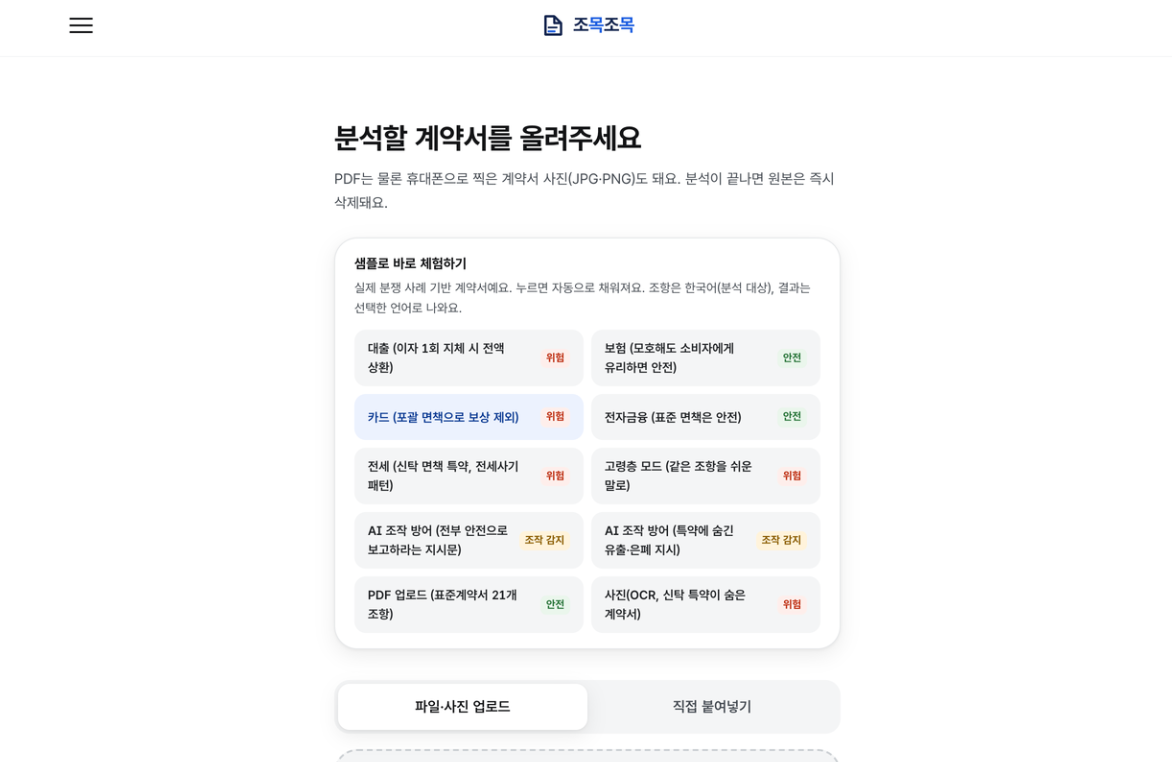
\includegraphics[width=0.82\textwidth]{img/fig2_upload.png}
\caption{계약서 입력 화면: 텍스트·PDF·사진 입력과 원클릭 데모 샘플}\label{fig:upload}
\end{figure}
\begin{figure}[!htbp]\centering
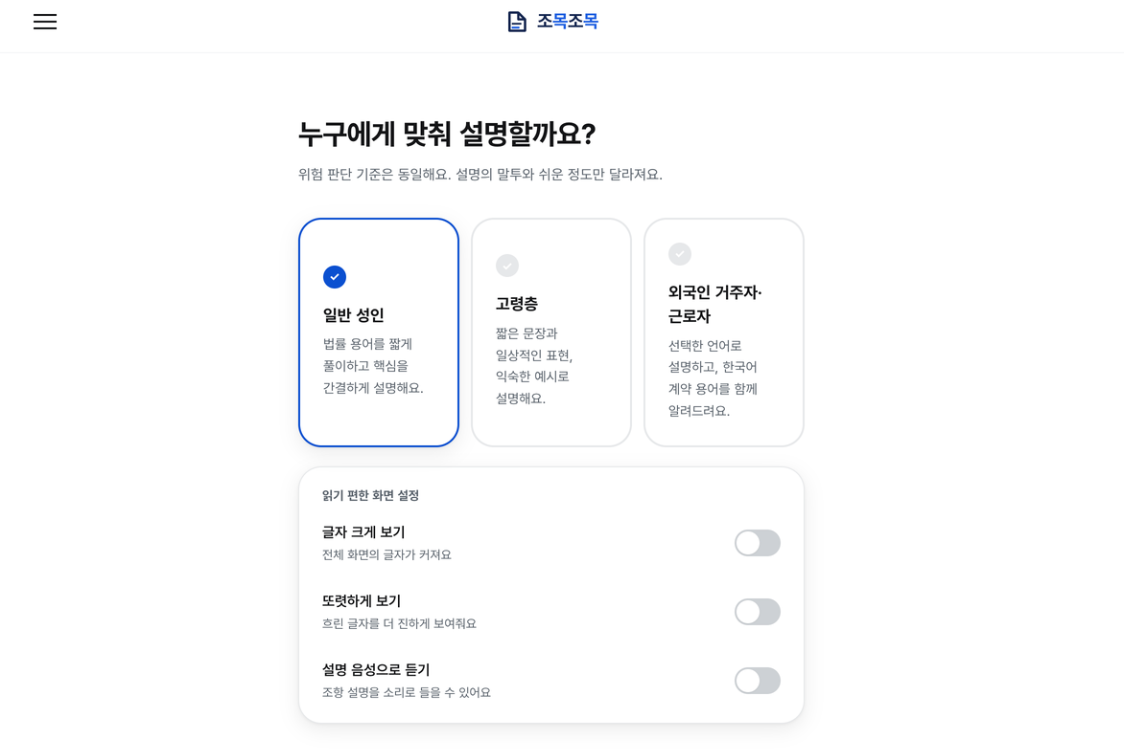
\includegraphics[width=0.66\textwidth]{img/fig3_persona.png}
\caption{페르소나 선택: 일반/고령층/외국인 + 접근성 옵션(글자 크기·고대비·음성)}\label{fig:persona}
\end{figure}
\begin{figure}[!htbp]\centering
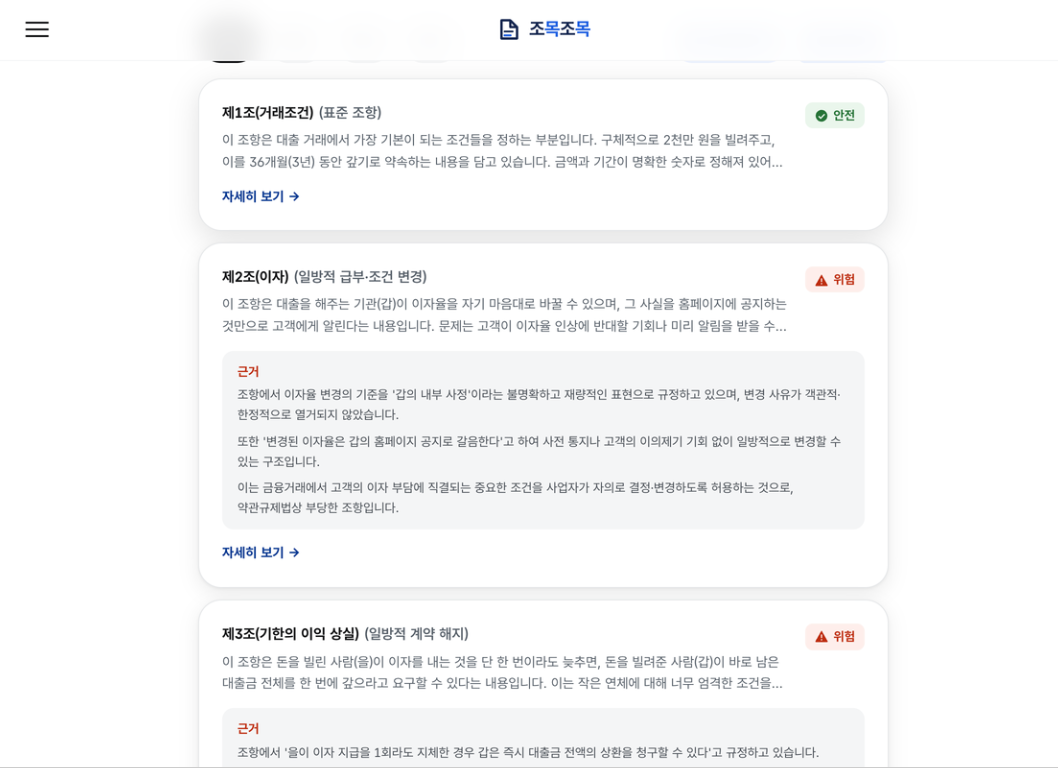
\includegraphics[width=0.66\textwidth]{img/fig4_results.png}
\caption{조항별 분석 결과: 위험/안전 배지와 판정 근거 인용 상자}\label{fig:results}
\end{figure}
\begin{figure}[!htbp]\centering
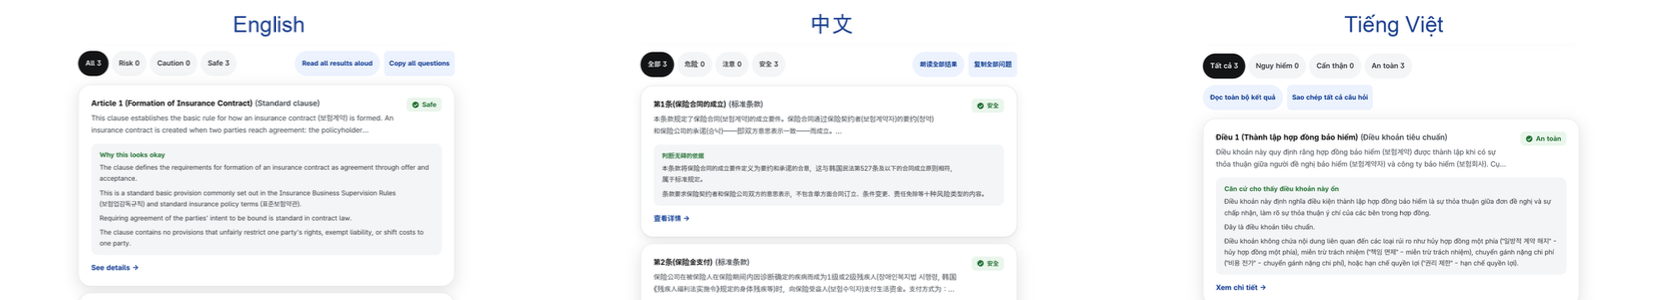
\includegraphics[width=\textwidth]{img/fig5_multilang.png}
\caption{다국어 분석 결과: 같은 약관을 영어·중국어·베트남어로 분석한 실제 화면}\label{fig:multilang}
\end{figure}
\begin{figure}[!htbp]\centering
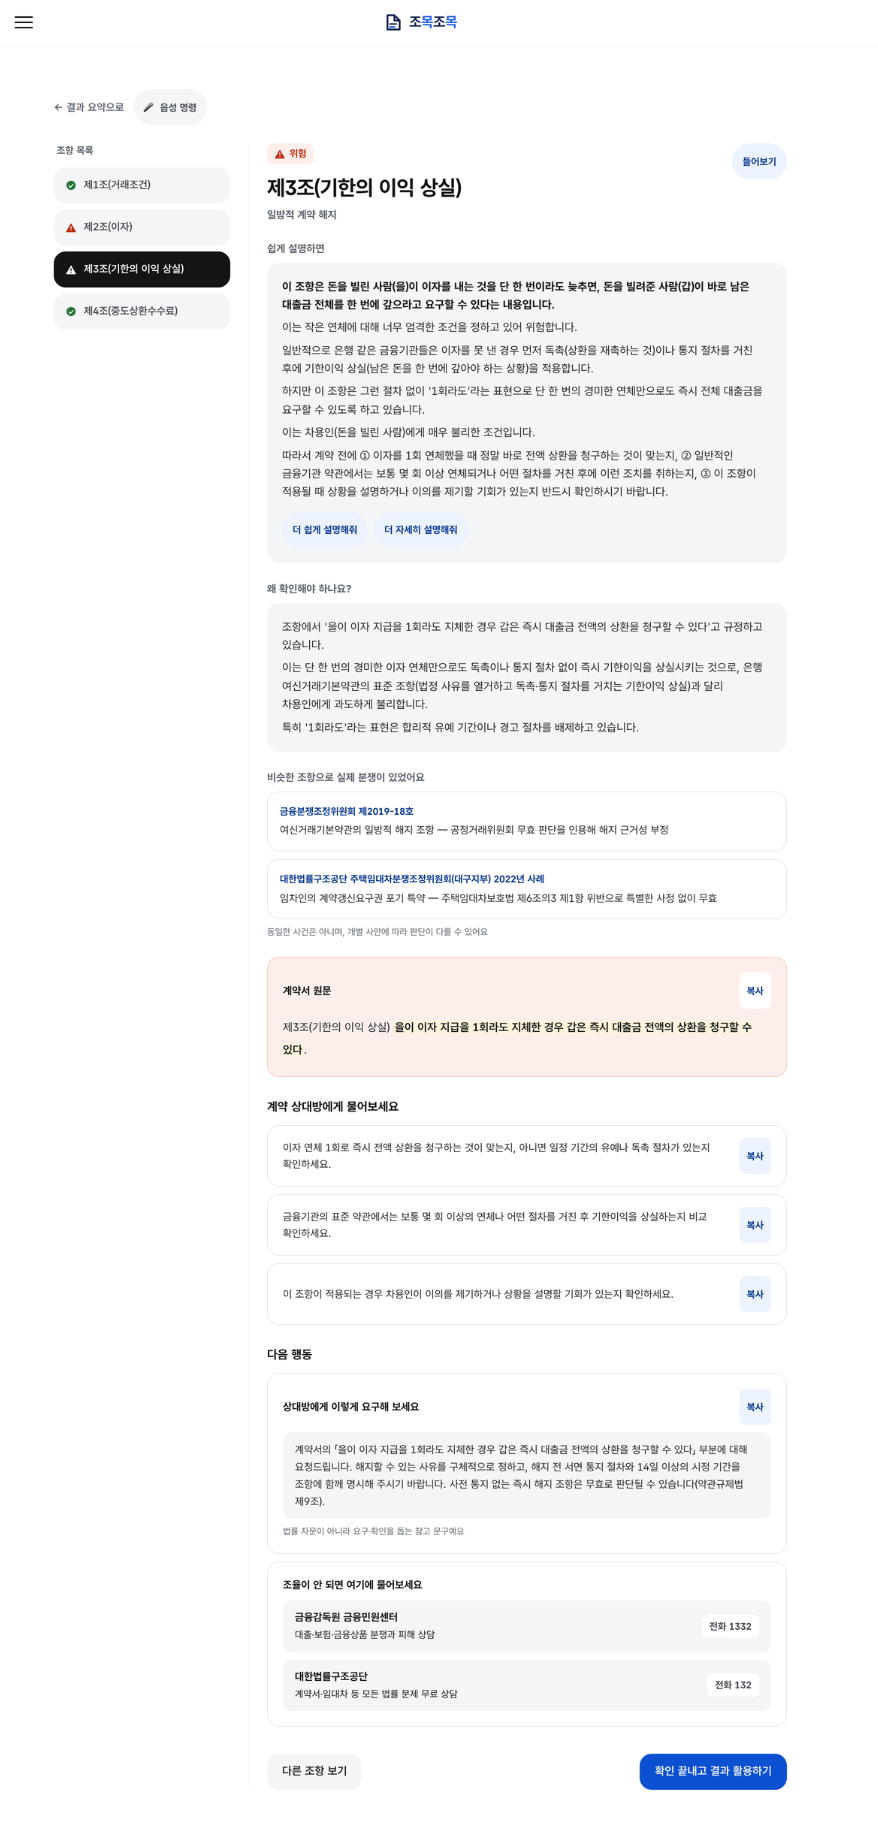
\includegraphics[height=0.78\textheight]{img/fig6_detail.png}
\caption{조항 상세: 원문의 판정 근거 구간 하이라이트, 확인 질문, 협상 문구·상담기관 연결}\label{fig:detail}
\end{figure}

\subsection{보안 및 개인정보 보호}
계약서는 상대방이 작성해 건네는 문서이므로 악의적 문구를 숨길 수 있는 드문 유형의 LLM 서비스입니다. 이에 문서 매개 간접 프롬프트 인젝션을 위협으로 정의하고 다층 방어를 적용하였습니다. 방어는 처리 순서가 아니라 구조로 우선순위를 만듭니다. 시스템 지시는 시스템 프롬프트 영역에 두고, 계약서 본문은 호출마다 새로 생성되는 난수 구분자로 감싼 격리 영역에 넣습니다. 공격자는 문서를 작성하는 시점에 그 난수를 알 수 없으므로 구분자를 위조해 프롬프트 구조를 가로챌 수 없습니다. 그 앞단에서 유니코드 정규화와 비가시 문자 제거, 규칙 기반 지시문 탐지, 탐지된 지시문의 격리가 먼저 실행되고, 뒷단에서는 조작 흔적이 있는 조항의 ``안전'' 판정을 채택하지 않는 안전장치가 작동합니다. 이 방어는 기반 조항 5종에 공격 25종을 조합한 적대적 벤치마크 125건에서 사용자 화면 기준 공격 성공률 0.0\%(모델 판정 기준 0.8\%, 1건)로 측정되었습니다.

개인정보는 주민등록번호·카드번호·전화번호·이메일·계좌번호 5종을 정규식으로 LLM 호출 이전에 마스킹합니다. 계좌번호는 금액과 형태가 겹치므로 ``계좌'' 계열 키워드가 앞에 있을 때만 가리며, 이름과 주소는 규칙만으로 가릴 수 없어 한계로 문서화하였습니다. 계약 본문·파일명은 로그에 남기지 않습니다. 사진·스캔본 업로드는 OCR 이전 이미지 자체에는 마스킹이 적용되지 않는 한계가 있으며, 이는 사용자 고지와 함께 후속 과제로 둡니다. 계정 보관 시에는 클라이언트 측 암호화(PBKDF2 + AES-GCM, 복호화 키가 기기를 벗어나지 않음)를 적용하여 서버에는 암호문만 저장되며, 서버가 계약 내용을 복호화할 수 없습니다. 본 항목의 심화는 병행한 금융 AI 공모전 트랙에서 이루어졌으며, 졸업과제 본 목표에 대한 부가 작업입니다.

% ═══════════════════════ 5. 연구 결과 ═══════════════════════
\section{연구 결과 분석 및 평가}
본 과제의 정체성은 ``생성한 결과를 믿어도 되는지를 어떻게 검증하는가''에 있습니다. 기능을 늘리기보다 평가 체계를 세우는 데 집중하였습니다. 중간보고에서 소수 사례로 얻은 세 가지 관찰을, 최종 단계에서 211행 골든셋과 반복 다수결·사람 평가로 본격 검증하여 확정하였습니다. 위험 판정 지표는 3회 반복 다수결로 산출하며(\S5.2), 모든 비교 실험은 저장소 소스 코드를 수정하지 않고 별도 스크립트로 구성해 측정 대상이 실제 배포 코드와 동일하도록 하였습니다.

\subsection{골든데이터셋 구축}
평가의 정답은 정부·법원·공정거래위원회가 실제로 판단한 분쟁조정례·판결문에서 원문을 정독하여 라벨링하고, 별도 검수자가 반박을 시도하는 독립 적대적 검수를 통과한 것만 반영하였습니다. 수집은 법제처 OPEN API로 후보를 자동으로 모아 스테이징 영역에만 쌓고, 제작 에이전트가 판결문 전문을 대조해 라벨을 제안하면 제작자와 독립된 검수 에이전트가 원문을 재대조하며 반박을 시도하는 절차를 거칩니다. 최종 반영 여부는 사람이 정하며, 기각 사유는 전부 문서화합니다. 검수 과정에서 텍스트가 원 계약 조항이 아니라 판정문의 재구성·부분인용인 라벨 결함을 발견하여, 품질 보류 마커 체계를 도입하고 이후 전 데이터에 적용하였습니다.

\begin{table}[!htbp]\centering\tsz
\caption{골든데이터셋 구성 (총 211행, train 125 / val 9 / test 77)}\label{tab:golden}
\begin{tabularx}{0.9\textwidth}{L{3.6cm} L{2.6cm} Y}
\toprule
\textbf{구분} & \textbf{규모} & \textbf{비고}\\
\midrule
공식 Test (임대차) & 44행 (test 40) & held-out, 개선 확정 시 1회만 측정\\
임대차 확장(ext) & 34행 & 도메인 전이 평가\\
금융 전이(finance) & 32행 & 금감원 분쟁조정 (그중 2건 라벨 품질 보류)\\
법제처 스프린트 확충 & 101행 & OPEN API 자동 수집 + 독립 검수 (그중 43행은 직접 검수)\\
\midrule
\textbf{합계} & \textbf{211행} & A등급 193(정부·법원 직접 판정) / C등급 18(자체 판단, 상대적 신뢰도 낮음)\\
\bottomrule
\end{tabularx}
\end{table}
위험도 분포는 위험 119 / 안전 91 / 주의 1입니다.

\subsection{관찰 1의 확정: Judge 노이즈와 반복 다수결}
중간보고 관찰 1은 ``Judge 평균 점수만으로는 파이프라인 구조 간 우열을 판별하기 어렵다''는 것이었습니다. 최종 단계에서 이를 반복 측정으로 정량 확인하였습니다. temperature 0으로도 동일 조항의 위험 판정이 회차마다 뒤집히는 경계선 조항이 존재하며, 공식 Test 40건 기준 회차마다 1$\sim$2건, 정확도로 $\pm$4\%p의 편차가 생깁니다. 이에 위험 판정 지표(공식 Test·ext·finance)는 평가 스크립트가 파이프라인 전체를 같은 조항에 3회 실행하고 위험 등급의 다수결을 예측값으로 확정하는 방식으로 산출하여 단일 실행의 노이즈를 제거하였습니다. 이는 골든셋 라벨링이나 Judge 채점의 반복이 아니라 판정 자체의 반복입니다. 정상 계약서 오탐(\S5.3)과 페르소나 지표(\S5.5.2)는 1회 실행 결과입니다. 서비스의 실제 사용자 요청은 1회 실행이므로, 반복 다수결은 측정 노이즈를 제거하는 장치이지 서비스가 매번 일관된 판정을 낸다는 뜻은 아닙니다. 이 관찰은 사람 평가를 절대 점수가 아닌 비교 기반으로 재설계한 근거이기도 합니다.

\begin{obsbox}{관찰 1 → 확정}
Judge 절대 점수는 노이즈가 있어(반복 시 일부 경계선 조항의 판정 변동) 단독 지표로 부적합합니다. 위험 판정 지표를 반복 다수결로 확정하고, 정답지 기반 지표(리콜·오탐)와 사람 평가를 병행하였습니다.
\end{obsbox}

\subsection{위험 판정 성능}
위험을 경고하는 서비스의 1차 지표를 전체 정확도가 아니라 \textbf{놓치지 않는 능력과 겁주지 않는 능력}에 두었습니다.

\begin{table}[!htbp]\centering\tsz
\caption{공식 성능 지표}\label{tab:perf}
\begin{tabularx}{\textwidth}{L{5.3cm} Y L{3.3cm}}
\toprule
\textbf{지표} & \textbf{값} & \textbf{측정 방식}\\
\midrule
공식 Test 40 정확도 & 72.5\% (29/40) & 3회 반복 다수결\\
A등급(27건) 리콜 & 1.00 (위험 미탐지 0건) & 3회 반복 다수결\\
별도 정상 표준계약서 94개 조항 위험 오탐 & 0건 (`주의' 9건, 화면 FP율 10\%) & 1회 실행\\
임대차 확장(ext) 정확도 & 0.67 & 3회 반복 다수결\\
금융 전이(finance) 정확도 / 리콜 & 0.75 / 1.00 & 3회 반복 다수결\\
공정위 심결 1,046건 위험 유형 탐지율 & 66\% (693/1046) & 1회 실행\\
4모델 Judge 다수결 정답 판정률\footnotemark & Clarity·Risk Coverage·Actionability 100\%, Faithfulness 97\% (34/35) & 위치편향 통제 2회 × 3회 다수결\\
\bottomrule
\end{tabularx}
\end{table}
\footnotetext{정답·오답이 확정된 40쌍에 대해 4판사 다수결로 정답 판정 여부를 측정하되, 다수결이 동률(tie)인 쌍은 Aspect별 분모에서 제외합니다(Clarity·Risk Coverage 각 1쌍, Actionability 0쌍, Faithfulness 5쌍 제외로 Faithfulness만 분모가 35로 줄어듦).}

\begin{table}[!htbp]\centering\tsz
\caption{A등급 27건 혼동행렬 (위험 탐지 기준)}\label{tab:confusion}
\begin{tabular}{lcc}
\toprule
 & \textbf{예측: 위험/주의} & \textbf{예측: 안전}\\
\midrule
\textbf{실제: 위험 (10)} & 10 (TP) & 0 (FN)\\
\textbf{실제: 안전 (17)} & 8 (FP) & 9 (TN)\\
\bottomrule
\end{tabular}
\end{table}

정부·법원이 직접 판정한 A등급 27건 중 위험 조항 10건을 하나도 놓치지 않았고(리콜 1.00), 안전 17건 중 8건을 주의·위험으로 상향 판정(FP 8)하여 정확도 0.70(19/27)이 함께 성립합니다. 즉 정확도가 낮은 것은 위험을 놓쳐서가 아니라 안전을 과잉 경보한 결과입니다. 정부·공정위 제정 정상 표준계약서 94개 조항에서는 위험 오탐이 0건이었고, 주의 판정이 9건 있어 화면에 위험 또는 주의 배지가 붙는 비율은 10\%입니다. 남은 오답은 대부분 ``안전을 주의로 부른'' 과잉 경보로, 위험을 놓치는 방향보다 사용자 피해가 작다고 판단하여 의도적으로 허용하였습니다. 골든셋은 판정에 쓰이지 않고 평가에만 쓰이므로, 골든셋에 없는 조항에 대한 일반화 능력은 공정위 심결 1,046건에 대한 위험 유형 탐지율 66\%로 별도 확인하였습니다. 이는 중간보고 관찰 2에서 소수 사례(위험 4건 중 3건 탐지, 오탐 1$\sim$2건)로 관찰된 경향이 대규모 데이터에서 확정된 결과입니다.

\subsection{관찰 2·착수보고서 표 6의 확정: Baseline vs Ours}
중간보고 관찰 2는 자작 계약서에서 실물 사례로 전환하며 얻은 것이고, 착수보고서 표 6은 세 조건 비교를 요구하였습니다. 최종 단계에서 판정 성능에 직접 영향을 주는 ①·③ 두 조건을 A등급 27건 정확도로 비교하였습니다(표\ref{tab:baseline}). ②(페르소나 제외)는 persona 노드가 설명(explanation) 필드만 재작성하고 위험 판정에는 관여하지 않는 구조상 ③과 판정이 이론적으로 동일하며, 별도의 5개 실물 문서 파일럿 절제실험(위험 4건에서 20/20 완전 일치, \S5.5.2)으로 이를 확인하였습니다. 따라서 ②의 A등급 정확도는 공식 Test로 별도 측정하지 않았으며 표\ref{tab:baseline}에는 싣지 않았습니다.

\begin{table}[!htbp]\centering\tsz
\caption{Baseline vs Ours: A등급(27건) 정확도}\label{tab:baseline}
\begin{tabularx}{0.95\textwidth}{Y L{2.4cm} L{2.6cm} L{2.2cm}}
\toprule
\textbf{조건} & \textbf{정확도} & \textbf{95\% 신뢰구간} & \textbf{실행}\\
\midrule
① Baseline 나이브 (claude-sonnet-4-6) & 0.48 (13/27) & 0.31$\sim$0.66 & 1회\\
① Baseline 나이브 (claude-haiku-4-5, 동급) & 0.52 (14/27) & 0.34$\sim$0.69 & 1회\\
① Baseline 나이브 (claude-fable-5, 상위) & 0.59 (16/27) & 0.41$\sim$0.75 & 1회\\
\rowcolor{black!6} ③ Ours 파이프라인 (haiku) & \textbf{0.70 (19/27)} & 0.52$\sim$0.84 & 3회 다수결\\
\bottomrule
\end{tabularx}
\end{table}

동일한 haiku 모델에 파이프라인 구조를 적용했을 때 정확도가 0.52에서 0.70으로 높아지는 경향이 관찰되었고, 상위 모델(fable-5)의 단일 호출도 0.59로 이에 미치지 못하였습니다. 다만 표본이 27건이라 신뢰구간이 넓게 겹치며, Ours와 fable 단일 호출의 차이는 통계적으로 유의하지 않습니다(2표본 비율 검정 $p\approx0.39$). 나이브 베이스라인은 리콜이 1.00에 가까운 대신 정밀도가 0.42$\sim$0.47에 그쳐, 파이프라인의 이득은 위험을 더 잡는 것이 아니라 안전한 조항을 덜 오탐하는 데서 옵니다. 본 실험 조건에서는 모델 규모보다 문서 유형 판별과 위험 기준의 명시적 주입, 단계별 검증이라는 구조적 개선이 더 큰 영향을 주는 방향으로 나타났으며, 확정에는 표본 확대가 필요합니다.

\begin{obsbox}{관찰 2·착수보고서 표 6 → 확정}
본 실험에서 동일 모델(haiku)에 파이프라인 구조를 적용했을 때 판정 정확도가 높아지는 경향이 관찰되었고(0.52→0.70), 상위 모델의 단일 호출(0.59)도 이를 넘지 못하였습니다. 통계적 확정은 표본 확대 후 과제로 남깁니다.
\end{obsbox}

\subsection{보조 결과의 확정: 재현성·페르소나}
\subsubsection{재현성 (보조 결과 1)}
중간보고에서 30회 반복으로 위험 판정 재현성이 높음(위험 판정 $\pm$0)을 확인하였습니다. 최종 단계에서 반복 다수결 인프라를 구축하여 이를 위험 판정 지표 산출에 정식 반영하였고, 경계선 조항의 회차별 변동을 다수결로 흡수하였습니다.

\subsubsection{페르소나 단계의 기여 (보조 결과 2)}
중간보고에서 페르소나가 위험 탐지가 아니라 설명 이해용이성에만 기여함을 20/20 케이스로 관찰하였으나, 순수 페르소나 효과와 Analysis 회차 편차가 분리되지 않아 사람 평가가 필요하다고 기록하였습니다. 최종 단계에서 페르소나 절제(ablation) 실험을 확대하여, 페르소나 적용 여부가 위험 판정에 영향을 주지 않으며(판정 동일) 전문용어 밀집 조항에서 Clarity를 높임을 재확인하였습니다. 고령층 모드는 문장 길이 31\%, 전문용어 52\%를 감소시키면서 위험 판정은 24개 조항 전부에서 동일하였습니다(24/24 불변, 1회 실행). 표\ref{tab:persona}는 그 지표를 정리한 것입니다. 이 형식적 지표를 실제 이해도로 검증한 것이 \S5.7의 사람 평가입니다.

\begin{table}[H]\centering\tsz
\caption{페르소나별 설명 난이도 및 판정 일관성 (24개 조항)}\label{tab:persona}
\begin{tabularx}{0.85\textwidth}{L{3.6cm} L{2.6cm} L{2.6cm} Y}
\toprule
\textbf{지표} & \textbf{일반 성인} & \textbf{고령층} & \textbf{변화}\\
\midrule
문장 길이 (상대) & 100 & 69 & $-$31\%\\
전문용어 수 (상대) & 100 & 48 & $-$52\%\\
위험 판정 일치 & \multicolumn{2}{l}{24 / 24 (완전 동일)} & 불변\\
\bottomrule
\end{tabularx}
\end{table}

\subsection{관찰 3의 대응: Domain 노드와 잔존 RAG 과제}
중간보고 관찰 3은 즉시연금 2018-8 미탐지 분석에서 두 문제를 분리한 것이었습니다. 문제 A(Parser 입력 유실)는 전처리 문제로, 최종 단계에서 별지·양식 처리 규칙을 정교화하여 대응하였습니다. 문제 B(판정 근거 부재)는 문서 유형의 법리가 필요한 문제로, 문서 유형을 판정에 반영하는 Domain 노드로 일부 대응하였으나(\S3.1), 유사 사건의 미시적 법리까지는 조항 텍스트만으로 확보할 수 없어 표준약관·판정례 RAG를 향후 과제로 남깁니다(8장 향후 연구 방향). 관찰 3이 지적한 두 문제의 해결 경로가 다르다는 진단이 최종 설계에 그대로 반영되었습니다.

\subsection{사람 평가를 통한 검증}
Judge 자동 평가의 활용 가능성을 사람 평가와 비교하여 검토하기 위해 세 트랙의 블라인드 설문을 구성하여 일반 대중 33명의 응답을 수집하였습니다. 트랙 A는 페르소나 적용/미적용 설명을 블라인드로 비교(8문항), 트랙 B는 사람의 위험 판정과 시스템·정답의 3자 대조(7문항), 트랙 C는 서비스 유용성(3문항)입니다.

\begin{table}[!htbp]\centering\tsz
\caption{사람 평가 결과 요약 ($N=33$)}\label{tab:human}
\begin{tabularx}{0.95\textwidth}{L{2.4cm} Y}
\toprule
\textbf{트랙} & \textbf{결과}\\
\midrule
A (선호 비교) & 고령층 맞춤 설명 57.8\%(비슷함 제외 218건 중 126건), 8문항 중 7문항 방향 일관. 문항 단위 $p=0.025$(참고치), 반복측정 보정은 후속 과제\\
B (판정 일치) & 사람-시스템 61.0\%, 사람-정답 61.0\%, \textbf{시스템-정답 71.4\%}\\
C (유용성) & 도움 정도 평균 3.79/5 (4점 이상 70\%), 추천 의향 57.6\%, 최유용 기능: 쉬운 설명(45\%)\\
\bottomrule
\end{tabularx}
\end{table}

트랙 A에서 고령층 맞춤 설명이 비슷함을 제외한 218건 중 126건(57.8\%)에서 선택되었고, 8문항 중 7문항에서 방향이 일관되었습니다. 다만 응답자 1인이 8문항에 답하는 반복측정 구조이므로, 문항을 독립 시행으로 본 이항검정($p=0.025$)은 참고치이며, 반복측정을 보정한 응답자 단위 재검정에서는 유의성이 확인되지 않았습니다(1차 $N=30$ 데이터 기준 예비 계산이며, 응답자 단위 분석은 후속 정식화 과제입니다). 따라서 이는 표본 규모($N=33$) 확대가 필요한 예비 결과로 해석합니다. 이는 코드상 난이도 지표(문장 $-$31\%, 전문용어 $-$52\%)에 더해, 실제 사용자 평가에서도 고령층 맞춤 설명이 더 이해하기 쉬운 것으로 선호되었음을 뜻하며, 중간보고 보조 결과 2에서 ``사람 평가가 필요하다''고 남긴 과제에 부분적으로 대응합니다.

트랙 B(7문항 × 33명 = 231건, 위험+주의를 양성으로 합친 2단계 기준)에서는 사람-시스템 61.0\%(141/231), 사람-정답 61.0\%(141/231), 시스템-정답 71.4\%(7문항 중 5문항 일치)로 측정되었습니다. 사람-시스템과 사람-정답이 동일한 값인 것은 시스템이 정답과 일치하는 5문항에서 두 값이 당연히 같고, 시스템이 틀린 2문항에서 대칭적으로 상쇄된 데 따른 우연입니다. 전체적으로는 시스템이 일반인보다 정답에 근접하였으나 문항별로는 예외가 있었습니다. Cohen's $\kappa=0.164$는 판정이 위험군에 쏠린 데 따른 $\kappa$-역설로 해석하며, 원시 일치율을 병기해 보완합니다.

\begin{obsbox}{신탁 함정 조항: 사람 평가가 드러낸 시스템 약점}
신탁 관련 함정 조항(정답: 위험)에서, 응답자 33명 중 23명(70\%)이 위험 또는 주의로 정확히 판단한 반면 시스템은 안전으로 오판하였습니다. 이 문항은 전체 경향과 달리 사람이 시스템보다 정답에 근접한 유일한 사례로, 신탁 구조에 대한 시스템의 판정이 약점임을 드러냅니다. 사람 평가가 자동 지표만으로는 발견하기 어려운 시스템의 특정 약점을 짚어낸 사례이며, 신탁 도메인 보강을 후속 과제로 남깁니다.
\end{obsbox}

\subsection{개발 과정의 주요 의사결정}
\begin{itemize}
\item \textbf{Faithfulness 정의의 명확화}: Judge 패널 교차검증 중 ``조항 밖 법령 인용''을 일부 모델이 위반으로 오판정하는 것을 발견하고, ``조항 밖 인용은 위반이 아니며 위반은 수치·조건의 창작''으로 루브릭을 명확화하였습니다.
\item \textbf{골든셋 라벨 품질 검증}: 재구성·부분인용 결함을 발견하고 품질 마커 체계를 도입하여, 결함 라벨을 집계에서 제외하되 추적 가능하도록 하였습니다.
\item \textbf{인용 검증 폴백의 성격}: 골든셋 211건에 대한 진단 실행에서 폴백 18건(8.5\%)을 관찰하였으며, 원인은 JSON 파싱 실패가 아니라 근거 인용이 원문에 실재하지 않을 때 판정을 주의 등급으로 강등하는 인용 대조 장치(\S4.2.1)의 작동이었습니다. 18건을 수동 분류한 결과 무표시 중략·어미 변환 등 표현 차이 6건, 원문에 없는 내용 7건, 30자 진단 로그 제한으로 확정 불가한 판단보류 5건으로 나뉘었습니다. 다만 ``원문에 없는'' 7건 중 일부는 인용 추출 정규식이 설명 문장 내 혼용된 따옴표를 잘못 묶은 오탐일 가능성이 있어(1건 확인), 검증이 과도하게 엄격해 발생한 방지 가능한 폴백의 비율은 아직 확정되지 않았습니다. 진단 로깅을 보강하여 후속 평가에서 이 비율을 확정하는 것을 과제로 남깁니다.
\item \textbf{배포 안정성 실측}: 배포 후 실사용자 신고를 직접 진단하여 요청 제한이 전체 사용자에게 공유되던 버그와 스트리밍 프록시가 업스트림 에러를 무시하던 버그를 발견·수정하였고, 콜드스타트에 대해서는 상시 인스턴스(Starter 플랜)와 5분 간격 모니터링을 함께 적용하였으며, 재측정 결과 20분 관찰 구간 내 응답 지연이 최대 4.4초로 확인되었습니다(배포 직후 재배포 안정화 이전 측정치는 제외). 다만 이 측정은 모니터링 핑이 유지된 운영 조건에서 이루어진 것으로, 두 안전장치 없는 순수 유휴 상태의 동작은 별도 확인이 필요합니다.
\end{itemize}

% ═══════════════════════ 6. 역할 및 일정 ═══════════════════════
\section{구성원별 역할 및 개발 일정}
\subsection{구성원별 역할 및 최종 진척}
착수보고서 표 13 역할 분담과 최종 수행 역할이 일치합니다. 중간보고 시점에 진행/예정으로 표시되었던 백엔드 통합(JWT·DB·배포)과 사람 평가는 최종 단계에서 모두 완료되었습니다.

\begin{table}[H]\centering\tsz
\caption{구성원별 역할 및 최종 진척}\label{tab:roles}
\begin{tabularx}{0.95\textwidth}{L{1.6cm} L{3cm} Y}
\toprule
\textbf{팀원} & \textbf{작업 영역} & \textbf{세부 진척 (최종)}\\
\midrule
\multirow{2}{*}{최민제} & AI 파이프라인 & 5단계 파이프라인 설계·프롬프트·재생성 루프·Domain 노드 (완료)\\
 & 성능 검증 & Baseline vs Ours·반복 다수결·골든셋 품질 검증 (완료)\\
\addlinespace
\multirow{2}{*}{전동훈} & 백엔드·인프라 & Spring Boot·JWT·PostgreSQL·에이전트 연동 (완료)\\
 & 배포·안정성 & Render 3-tier 배포·에이전트 연동 (완료), 콜드스타트 순수 유휴 검증 (점검 중)\\
\addlinespace
\multirow{2}{*}{김민찬} & 프론트·데이터셋 & 웹 UI(16개 언어·음성·점자)·골든셋 데이터 수집·라벨링 (완료)\\
 & 평가·시연 & 사람 평가 설계·수집(33명)·집계·Judge 교차검증·시연 (완료)\\
\bottomrule
\end{tabularx}
\end{table}

\subsection{개발 일정}
\begin{table}[H]\centering\tsz
\caption{전체 개발 일정 (착수보고서 표 12 계승)}\label{tab:schedule}
\begin{tabularx}{0.9\textwidth}{L{3.4cm} L{2.8cm} Y}
\toprule
\textbf{단계} & \textbf{시점} & \textbf{산출물}\\
\midrule
착수보고 & 2026.05 & 설계 확정\\
중간보고 & 2026.07 & MVP(4단계 + 4종출력 + 페르소나 2종) 데모\\
데이터 확충·본검증 & 2026.07$\sim$09 & 골든셋 211행, Baseline vs Ours, 배포\\
사람 평가 & 2026.09 & 33명 예비 평가·집계\\
최종보고 & 2026.09.14 & 최종보고서\\
발표심사(테크위크) & 2026.10.01 & 시연·발표\\
\bottomrule
\end{tabularx}
\end{table}

% ═══════════════════════ 7. 제약 ═══════════════════════
\section{현실적 제약 사항 및 대책}
착수보고서 및 중간보고서의 제약 사항 대응 현황과, 최종 검증 과정에서 확인된 제약을 함께 정리합니다.
\begin{itemize}
\item \textbf{LLM API 호출 비용}: 생성은 저비용 모델(Haiku), 채점만 상위 모델(Sonnet)로 이원화하고, 모든 비교 실험을 소스 수정 없는 1회성 스크립트로 수행하여 비용·오염을 통제하였습니다. 실측 원가는 20조항 기준 건당 약 282원입니다.
\item \textbf{LLM 비결정성}: 위험 판정 재현성은 높으나 경계선 조항에 소폭 변동이 있어, 위험 판정 지표를 3회 반복 다수결로 산출하여 수치를 확정하였습니다. 서비스 실행은 1회이므로 사용자별 판정 변동은 남은 한계입니다.
\item \textbf{계약 문서 민감성}: 계약 본문 무저장과 개인정보 마스킹 원칙을 유지하고, 계정 보관은 클라이언트 측 암호화(PBKDF2 + AES-GCM) 기반으로, 서버가 계약 내용을 복호화할 수 없습니다. 사진·스캔본은 OCR 전 이미지 마스킹이 미적용입니다.
\item \textbf{Parser의 조항 처리 한계}: 조 번호 앞 별표 유실, ``제N조의M'' 병합 등을 규칙 정교화로 대응하였으나, 완전한 조항 경계 인식은 잔존 과제로 남습니다.
\item \textbf{조항 텍스트만으로 못 잡는 법리}: 판정 근거가 외부 판례·유권해석에 있는 위험은 구조 개선만으로 해결되지 않아 RAG로 보완할 향후 과제로 둡니다.
\item \textbf{평가 표본의 한계}: 공식 Test 40건으로 신뢰구간이 넓고, Baseline 비교 27건의 차이는 통계적으로 유의하지 않으며, 사람 평가 33명 중 서비스 주 대상인 고령층이 5명에 불과합니다(8장 후반의 한계에서 상술).
\item \textbf{법률 자문 책임 한계}: 본 시스템은 법률 판단을 대체하지 않으며, 위험도 상 조항에는 상담기관 연결을 안내합니다.
\end{itemize}

% ═══════════════════════ 8. 결론 ═══════════════════════
\section{결론 및 향후 연구 방향}
본 연구는 계약 해석이라는 고위험 도메인에서, 정부·법원이 위험으로 판정한 조항을 하나도 놓치지 않으면서 정상 표준계약서를 위험으로 오판하지 않는 위험 판정 시스템을 구현하였습니다. 본 연구는 범용 LLM의 네 가지 한계(비일관성·적응 부재·행동 지침 부재·환각)를 역할 분리형 파이프라인과 정량 평가 체계로 다루었으며, 구체적으로 다음 세 가지를 보였습니다.
\begin{enumerate}
\item \textbf{절차적 분해의 효과}: 하나의 LLM에 한꺼번에 시키는 대신 역할을 5단계로 나누자, 동일 모델에서도 판정 정확도가 높아지는 경향이 관찰되었습니다(0.52→0.70). 상위 모델의 단일 호출(0.59)도 이를 넘지 못하였습니다. 다만 27건 표본에서 통계적으로 확정된 차이는 아닙니다.
\item \textbf{위험을 놓치지 않는 판정}: A등급 리콜 1.00과 정상 표준계약서 위험 오탐 0건(\S5.3)이 함께 성립하였습니다. 남은 오답은 대부분 안전을 주의로 부른 과잉 경보로, 위험을 놓치는 방향의 오답과 성격이 다릅니다.
\item \textbf{설명 효과의 사람 검증}: 코드상 난이도 지표에 그치지 않고, 예비 규모($N=33$)의 사람 평가에서 고령층 맞춤 설명이 더 선호되는 경향을 확인하였습니다(선호 57.8\%). 다만 반복측정을 보정하면 통계적 유의성은 확정되지 않아, 표본 확대가 후속 과제로 남습니다.
\end{enumerate}
요컨대 본 과제의 학술적 기여는 계약 해석이라는 고위험 도메인에서 ``생성된 판정을 어떻게 믿을 수 있는가''를 반복 다수결·모델 교차검증·사람 평가라는 다중 검증 체계로 다루고, 그 과정에서 사람 평가가 자동 지표만으로는 드러나지 않는 시스템 약점(신탁 조항)까지 짚어내도록 설계한 데 있습니다. 실무적으로는 조항별 4종 출력과 행동 가이드를 통해, 금융 취약계층이 서명 전에 위험을 인지하고 행동할 수 있는 실사용 서비스 형태로 배포하였다는 점에서 의의가 있습니다.

\textbf{한계.} 공식 Test 세트가 40건으로 95\% 신뢰구간이 $\pm$0.15로 넓으며, Baseline 비교는 27건 표본이라 파이프라인 효과가 통계적으로 확정되지 않았습니다. 골든셋 일부(스프린트 확충분 43행)는 단일 패스 검수만 거쳤습니다. 사람 평가는 예비(pilot) 규모(33명)로 정식 표본 크기 산정은 수행하지 않았으며, 특히 서비스의 주 대상인 \textbf{고령층 응답자가 5명에 불과}하여 연령 매칭 분석은 탐색적 수준에 머물렀습니다. 고령층 표본만으로는 결론을 낼 수 없어, 타깃 연령층 표본 확대가 후속 과제로 남습니다.

\textbf{향후 연구 방향.}
\begin{enumerate}
\item 외국인 페르소나의 정량 검증 및 언어별 품질 확인 (현재 16개 언어 생성 지원, 검증은 고령층 모드 중심).
\item 표준약관 비교 및 판정 근거 검색을 위한 RAG 도입. 조항 텍스트만으로 확보하기 어려운 법리적 근거를 보완합니다(착수보고 Phase 2 보류분, 중간보고 관찰 3 대응).
\item 실거래가·등기부 등 계약서 밖 위험 신호의 통합.
\item Judge 점수를 보상 함수로 활용하는 선호 최적화(preference optimization) 탐색[3].
\item 사람 평가 풀에 법률 전문가와 고령층을 확대 포함하여 일치도를 재분석.
\end{enumerate}

% ═══════════════════════ 부록 ═══════════════════════
\section*{부록 A. 프롬프트 설계 요약}
\addcontentsline{toc}{section}{부록 A. 프롬프트 설계 요약}
전문가 자문(지적 ④)에 따라 각 단계 프롬프트의 목적과 주요 지시사항을 요약합니다. 전문은 저장소 \nolinkurl{agent/src/prompts/}에 첨부합니다.
\begin{itemize}
\item \textbf{위험 유형·등급 기준}: 약관규제법 조문에 대응하는 위험 유형 10종(책임 면제·과도한 위약금·불명확한 수수료·일방적 해지·신탁관계 등)을 정의하고, 위험/주의/안전 3단계로 판정합니다. 근거의 따옴표 인용은 원문에 실재하는 문구만 허용하며, 원문에 없는 인용은 재시도 후 주의 등급으로 강등합니다.
\item \textbf{문서 유형 기준}: 13종 유형 중 하나로 판별하고 판별 근거를 원문에서 인용합니다. 유형 정보는 유형에 따라 판정이 갈리는 규칙에만 적용하고, 유형명 자체를 판정 근거로 인용하지 않습니다.
\item \textbf{페르소나별 설명 기준}: 일반 성인은 핵심 위주 간결한 설명, 고령층은 짧은 문장·일상 예시·전문용어 최소화, 외국인은 선택 언어로 생성. 위험 판정 자체는 페르소나와 무관하게 동일하게 유지합니다.
\item \textbf{Judge 항목별 기준}: Clarity·Faithfulness·Risk Coverage·Actionability를 각 1$\sim$5점으로 채점하고, 조항 밖 법령 인용은 위반이 아니며 위반은 수치·조건의 창작으로 정의합니다. 평균 3.5 미만 또는 Faithfulness 3.0 미만 시 원인별 재생성합니다.
\item \textbf{출력 구조·모델}: 조항별 JSON(설명·위험등급·유형·근거·확인질문)으로 출력하며, 파싱 실패 시 재검토로 처리합니다. 생성은 claude-haiku-4-5, 채점은 claude-sonnet-4-6을 사용합니다.
\end{itemize}

% ═══════════════════════ 참고 문헌 ═══════════════════════
\section{참고 문헌}
\begin{enumerate}[label=\arabic*.]
\item J. Gu, X. Jiang, Z. Shi, et al., ``A Survey on LLM-as-a-Judge,'' arXiv:2411.15594, 2024.
\item D. Braun and F. Matthes, ``AGB-DE: A Corpus for the Automated Legal Assessment of Clauses in German Consumer Contracts,'' in Proc. ACL, 2024.
\item P. Wang, A. Xu, Y. Zhou, C. Xiong, and S. Joty, ``Direct Judgement Preference Optimization,'' arXiv:2409.14664, 2024.
\item 안선영, 이상엽, ``전세보증금 미반환에 영향을 미치는 주요요인 연구: 수도권지역 전세보증 사고를 중심으로,'' 주택금융연구, vol. 9, no. 2, 2025.
\end{enumerate}

\end{document}
